\section{Clojure}
\begin{itemize}
\item Lenguaje del 2007.
\item Derivado del Lisp.
\item Es homoiconico, los programas se escriben usando las propias estructuras de datos del lenguaje. (podemos escribir código que interprete otro programa, por eso es bueno para interpretes, Clojure esta escrito en Clojure)
\item Es un compilador en tiempo real, da la impresión de ser un interprete, pero en realidad compila y después ejecuta.
\item Se traduce a byte code de java, es quien ejecuta realmente. Es parte de ese universo.
\item Es muy integrable y expresivo a proyectos grandes. Con poco código puedo obtener muchos resultados.
\item Leiningen, es un gestor de paquetes para Clojure.
\item En Clojure las variables son temporales.
\item Le da preferencia a la recursividad y funciones de orden superior (funciones que reciben y/o devuelven otras funciones).
\item Permite representar conjuntos potencialmente infinitos.
\item Ofrece una consola de evaluación (REPL: read eval print loop)
\item Los predicados en Clojure tienen nombres que terminan en signo de pregunta (?) \textit{Ej. even?} Se pueden ver con \mint{clojure}|(apropos "?")|
\item Importamos archivos REPL con \mint{clojure}|(load-file "nombre")| después ejecutamos el programa llamando a la primer función (main). Si queremos usar un proyecto es diferente. (Es un conjunto de funciones metidas en un archivo)
\item La primera posición la toma como una función. (deriva del concepto de aplicación de calculo lambda)
\end{itemize}


Estudiamos 6 partes en el curso:
\subsection*{Datos}
Un dato puede ser un escalar, una colección cuyos elementos son datos, o una secuencia (abstracción que representa una vista secuencial de una colección)

\subsubsection*{Escalares}

\begin{itemize}
\item Los símbolos se refieren a un único elemento, representan el nombre de algo (es Case Sensitive). No puedo tener nombres que empiezan con números. Si queremos evitar que evalué un símbolo incluimos un apostrofe a la izquierda del símbolo.  Ejemplo: \mint{clojure}| 'a |
\item Los valores literales pueden ser números (enteros como long o BigInt si tiene N como sufijo, punto flotante como double o BigDecimmal si tiene el sufijo M, racionales para fracciones). Los caracteres se representan con la barra invertida al lado del caracter (\textbackslash a). Hay cadenas de caracteres con comillas dobles ("hola mundo")
\item El nulo es el valor Ni, significa nada y representa una referencia nula.
\item Los valores de verdad true y false.
\item Tenemos constantes simbólicas como \#\#Inf, \#\#-Inf y \#\#NaN (depende la version)
\item Hay palabras clave para indexar valores de los mapas, deben empezar con dos puntos (:primero), no se les permite iniciar con un . a la palabra clave.
\end{itemize}

\subsubsection*{Colecciones}
\begin{itemize}
\item \textbf{Listas} se usan para representar código, van entre paréntesis. () es la lista vacía. Se usan para acceder secuencialmente a los datos, mantener el orden a medida que se insertan, mantener elementos repetidos, y para agregar y quitar datos rápidamente del frente (LIFO).
\item \textbf{Vectores} se usan para representar datos, van entre corchetes. [] es el vector vació. Se pueden usar comas para separar los datos.
\item Son útiles para acceder por índice aleatoriamente, mantener datos repetidos, mantener orden, y agregar y quitar rápidamente datos del final (LIFO)
\item \textbf{Colas} no tienen codificación literal. Se deben construir a partir de la cola vacía. Sirve para acceder secuencialmente, mantener repetidos, mantener orden a medida que se insertan, y agregar datos al final y quitar del frente rápidamente (FIFO)
\item \textbf{Conjuntos}, tenemos el hash-set y el sorted-set. Van entre llaves empezando con el numeral. (\#{}) Sirven para mantener datos sin repeticiones, agregar o eliminar un dato dado, verificar si existe un dato en el conjunto.
\item \textbf{Mapas} van con llaves sin el numeral. {:x 10,:y 15}. Acceso aleatorio a los datos por clave, agregar asociaciones de claves únicas y valores, eliminar pares, y verificar si existe una clave en el mapa. Existen hash-map y sorted-map
\end{itemize}


\subsubsection*{Secuencias}
\begin{itemize}
\item Mediante la interfaz ISeq tenemos funciones de propósito general para trabajar con secuencias. Una seq es una abstracción representando una vista secuencial de una colección, osea una lista lógica que proporciona un acceso estable a una secuencia de valores. 
\item Las listas concretas implementan ISeq, por lo que son secuencias.
\end{itemize}



\subsection*{Evaluación de expresiones}
Todo es una expresión que al ser evaluadas devuelven un valor.


\subsection*{Formas especiales}
Las formas especiales tienen reglas de evaluación que difieren de las reglas estándar. Su listado  completo se obtiene evaluando: \mint{clojure}|(pprint (keys (. clojure.lang.Compiler specials)))|.

\begin{itemize}
\item Un ejemplo es el if, no toma todos los argumentos, toma solo a medida que se va evaluando. (lazy evaluation)
\item Algunas funciones que tienen efectos colaterales (ej print) además de imprimir retornan nil. (Todo tiene que devolver algo)
\item let es para variables. Se liga el valor al identificador declarado. Esta permitido usarlo, es una especie de 'syntactic sugar'. \mint{clojure}|(let [a [1 2 3], b 4]| liga a al vector [1 2 3] y b a 4 . No deja efectos colaterales, si veo cuanto vale a, me va a dar indefinido (afuera de la función). Tratar de programar sin let provoca código largo y repetido.
\item Tenemos try-catch-finally
\item Las funciones que empiezan con un punto son un atajo a java. Es una forma especial. Si el primer operando es un  símbolo que se resuelve como un nombre de clase, se considera el acceso a un miembro estático de  la clase nombrada. Si el segundo operando es un símbolo y no se proporciona ningún argumento, se  considera que es el acceso a un atributo.
\end{itemize}



% scheme , usar internamente un toUpperCase para poder manejarse sin preocuparse si ingresaron mayus o no

%%%%%%%%
\subsection*{Funciones predefinidas}
Se tienen varias funciones predefinidas, se mencionan algunas.
\begin{itemize}
\item symbol devuelve un símbolo con el nombre indicado
\item Si quiero agregar un paréntesis o algún carácter especial de Clojure usaría symbol para que me de ese símbolo en especial. ej symbol ")"
\item number? es mas fácil ir preguntando con esta función que directamente con el tipo (ej integer?)
\item mod y rem son distintos. La diferencia se nota en los negativos. % elegir de acuerdo a como hace scheme para mostrar el resto.
\item str para convertir algo a una cadena. Si se le pasa mas de una cosa las concatena.
\item replace, si lo ponemos solo busca el que esta en core, pero le podemos especificar que queremos que use el de clojure.string
\item prn imprime tal cual la cadena, print analiza la cadena (ej los \textbackslash n)
\item Los números son todos true (truthfy) (incluido el 0), los falsos son nil y el propio false.
\item some? para preguntar si algo es distinto de nil
\item keyword construyo una palabra clave.
\item hash-map (no se cuantos argumentos va a tener, solo que la cantidad de argumentos va a ser par, sino se queja) y zip-map, la diferencia esta en que les paso para construir el mapa
\item contains? tiene diferentes implementaciones dependiendo de si se le pasa un vector, hash-set, o mapa
\item pop para quitar un dato de la colección, tener cuidado que la colección no se modifica.
\item get devuelve el elemento, se justifica respecto de (V pos) porque le podemos pasar un valor alternativo (get V 1 "me pase")
\item into es mejor con vectores, no los desordena
\item No olvidarse de que son inmutables.
\item frequencies esta buena para funciones estadísticas, te devuelve cuantas veces aparece algo en un mapa
\item (doc funcion) nos da la documentación de una función.
\item Con (seq coleccion) nos crea una secuencia a partir de distintas entradas.
\item Con (repeat argumento) devuelve una secuencia infinita repitiendo el argumento. Muy potente esta función.
\item Con (range) devuelve una secuencia monotona creciente de numeros a partir del 0. Se le puede indicar un rango tambien. Si queremos mas potencia todavia le podemos dar el step.
\item (rest coleccion) (next coleccion) para ir moviendose en una coleccion. (Devuelven la coleccion sin el primer elemento) (Difieren en lo que devuelven al final.)
\item Si queremos pedir el primero del primero, podemos usar (ffirst '(colecciones)) en lugar de (first (first '(colecciones))) Mirar Operaciones dobles para más detalles.
\item (drop ) para remover multiples datos.
\item (re-seq ) devuelve en una secuencia las subcadenas de una cadena que coinciden con una expresion regular. \textit{Muy importante para el TP}.
\item (count ) para el tamaño de una secuencia.
\item (concar ) para concatenar secuencias.
\item (flatten ) para planchar una secuencia.
\end{itemize}

% Scheme usa (car '()) y (cdr '())


\subsection*{Funciones de orden superior}
Son funciones que reciben a otras funciones. Usar estas funciones es más idiomática.

Poniendo el numeral adelante es una funcion anonima.

\begin{itemize}
    \item (apply funcion): invoca una funcion de aridad n con los n datos contenidos en el segundo. Podemos crear funciones de orden superior usando estas primitivas.
    \item (map funcion): Devuelve la secuencia formada por el resultado de aplicar una funcion.
    \item (mapv funcion): Igual que map solo que devuelve un vector.
    \item (partial funcion): Devuelve una funcion de menor aridad que la indicada por el primer argumento, fijamos argumentos.
    \item (reduce funcion): Aplica una funcion de aridad 2 al primer y segundo dato, luego el resultado se devuelve y es usado por el tercer dato, y así sucesivamente. No necesitamos agregar un 'tachito' como en FP para ir guardando los resultados.
    \item (filter funcion): permite seleccionar multiples datos. Devuelve una secuencia.
    \item (take-while funcion): Toma mientras se cumpla la condición
    \item (remove funcion): Devuelve una secuencia eliminando los datos del segundo argumento que cumplan con el predicado. (Lo opuesto de filter, se queda con los que no cumplen)
    \item (drop-while funcion): Opuesto a take-while
    \item (every? funcion): Devuelve si se cumple la condicion para todos los argumentos.
    \item (not-every? funcion): Devuelve si no todos cumplen la condicion.
    \item (not-any? funcion): Si hay por lo menos uno o no.
    \item (comp funcion): Devuelve una función que es la composición de los argumentos recibidos.
    \item (iterate funcion): Devuelve una secuencia infinita formada por el segundo argumento, seguido del primer argumento aplicado sobre el segundo. No se usa mucho. Hay que usar take para que termine.
    \item (sort funcion): Se le pasa el criterio de ordenamiento.
    \item (sort-by funcion): Ordena una secuencia con los datos del ultimo argumento, ordenados según los resultados de aplicar una función indicada. \textit{Ej. una secuencia con mapas.}
    \item (partition-by funcion) Devuelve una secuencia con los valores del segundo argumento particionados según el primero. Va de forma iterativa, crea particiones. No los desordena.
    \item (group-by funcion): Agrupa segun el argumento. Crea los grupos.
\end{itemize}


\subsection*{Macros predefinidas}

No los puedo usar con map. Si los quiero usar con map debo envolverlos en una funcion.
\begin{itemize}
    \item (cond condiciones y expresiones): Es mejor que el if, más cómoda. La ultima condición tiene que ser algo que sea truthfy (true, :else, :default) puede ser cualquier cosa. Se detiene en la primera que cumple la condición.
    \item (case n): Es como un switch. No tiene condiciones, segun cada caso devuelve lo que corresponda
    \item (and condiciones)
    \item (or condiciones)
    \item (for ): Es una sintaxis para expresar una lista por comprension.
    \item Hay tres tipos de flecha. $->$ , $->>$ , $->>>$, cada una aplica una serie de transformaciones sobre un conjunto . La ventaja es que lo puedo leer de forma mas clara.
    \item (with-out-str ) Es bueno para los tests. Evalúa expresiones y devuelve una cadena con la concatenación de sus salidas.
    \item (declare ) es igual a def, la diferencia esta que permite indicar varias funciones a la vez. Se usa para forward declarations.
\end{itemize}

\section*{Programación funcional - Clojure}


\begin{itemize}
\item Bastante funcional debido a que cumple con las 7 características
\item Programas como funciones. El programa consiste en la lista de definiciones de funciones, y la ejecución es aplicarlas.
\item Funciones puras. Determinismo, ante los mismos argumentos devuelve el mismo valor (random no es pura), y ausencia de efectos colaterales.
\item Datos inmutables, no modifica los valores, cambia las copias.
\item Funciones de primera clase, se pueden pasar como argumento.
\item Funciones de orden superior, toman funciones como argumento o las retornan.
\item Composición de funciones, clojure permite componer funciones de diversas maneras. comp, partial, flechas
\item Recursividad, clojure permite con pila y sin pila (recur para que la use si esta disponible).
\end{itemize}

\section{Interpretes}
% SCM interprete de scheme en el que tenemos que inspirarnos
% esta prohibido usar def DENTRO del cuerpo de las funciones en el TP


\begin{itemize}
\item Podemos hacer un interprete del lenguaje que queramos.
\item Siempre hay necesidad de nuevos lenguajes. Esto se conoce como abstracción metalingüística.
\item El interprete es otro programa, estamos usando un lenguaje para crear un programa que interpreta otros programas.
\item Scheme es un lenguaje funcional, esta pensado para evaluar expresiones.
\item Segun el significado del operador en la primera posicion le hago hacer algo.
\end{itemize}

\begin{figure}[!htb]
    \centering
    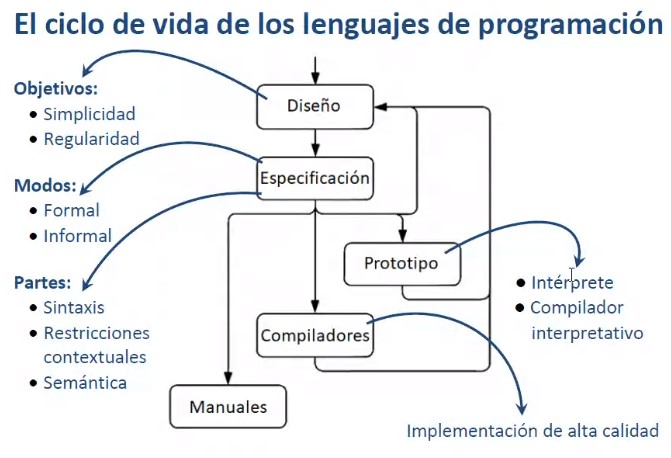
\includegraphics[width=0.8\textwidth]{img/CicloDeVidaLenguajes.jpg}
\end{figure}


\begin{itemize}
\item En Scheme el valor booleano true es \#t, y el false \#f.
\item Procesadores de lenguaje, cualquier sistema que manipule programas expresados en algún lenguaje. Sirven para ejecutar programas o prepararlos para ser ejecutados.
\end{itemize}
% proteger-bool-en-str, agrega % a los numerales ( # -> % )
% read-string convierte a una lista de clojure
% no tenemos que hacer el scanner, clojure convierte el string en una estructura, solo falla con los #
% evaluar trabaja con una estructura de datos, una representacion intermedia - ri -
% se va actualizando el ambiente, scheme no es un lenguaje puro, modifica el ambiente. En el interprete llamamos devuelta al repl

\begin{itemize}
\item Hay problemas prácticos de la interpretación, el rendimiento y el requerimiento de memoria.
\item Compilación interpretativa, un compilador genera código de maquina y un interprete emula su ejecución. (Ej. Java)
\end{itemize}
% read-line es el scanner

% diplay para que nos imprima por pantalla al cargar el archivo
% la propia accion de cargarlo carga las funciones y lo prueba

% Problema de las 2 jarras, tengo una de 5l y otra de 8l, necesito una con 4l. No estan graduadas
% Planteamos las transiciones y cambios validos y lo ponemos a evaluar
%

% Dividimos entre si es funcion o no en nuestro interprete (evalua todo o no, si no evalua todo en clojure seria una macro o forma especial)

% no realizar converciones innecesarias en el interprete
% sin define el set! tira error, no se puede hacer set! a una variable que no esta ligada


% scheme sirve para programas que ocupen poco espacio
% main llama al (repl)
% with-in-str para probar la entrada en leer
% no entregar el jar